\chapter{Thermal conductivity simulations of Silica glass}

\LEnote{*** INTRODUCTION, STATO DELL'ARTE ***}

\paragraph{Thermal conductivity of glasses}
Thermal conductivity of glass systems is a fundamental property for many industrial and technological applications, \emph{e.g.} heat management in electronic devices, windows for green architectures.
However, ``thermal conductivity represents largely explored territories, ripe for new research efforts'' [J.Mauro...]\cite{MauroFM14,Mauro2014}. The understanding of thermal conductivity and its structural origin in glasses has been greatly overlooked in the literature. 

\paragraph{Vitreous silica}
Vitreous silica has been the subject of significant research efforts in the last decades, due to is many technological applications that range from thermal insulation to laser engineering, semiconductor fabrication, and optical communication.
In particular, thanks to its excellent UV transparency, mechanical stability, and chemical durability, silica can be used in many optical applications, such as the diffractive elements and the protective windows of the optics assemblies of inertial confinement fusion facilities. In these facilities, extremely intense nanosecond laser pulses are used and seriously challenge the durability the optical glasses. It is indeed well established that the small defects or impurities of the glass may induce damage craters due to local lattice heating and melting, that will result in a rapid optical degradation \cite{Miller2004,Canaud2004,Miller2010,Chambonneau2014,Kuzuu1999,Stuart1995,Wong2006,Carr2010,Saito2000}. The interpretation of this damage process requires the study of thermal transport and the prediction of the thermal conductivity. 

Furthermore, amorphous silica serves as the basis of multicomponent silica glasses, that are adopted for a wide range of special applications. 
Therefore predicting the thermal conductivity of silica is the first step to predict the thermal conductivity of more complicated glasses, whose elements are characterized by a complex chemistry that is difficult to model.

**Esempio vetri borosilicati ecc**

\LEnote{**AEROGELS: \small Silica aerogel, a highly porous material first synthesized in the
early thirties [1], are currently being produced using a sol–gel process
such as hydrolyzing tetramethoxysilane (TMOS) to form silica and
methanol, and subsequently dried through supercritical drying together
with carbon dioxide [2]. Silica aerogel has several highly desirable
properties including being environmentally safe, having high optical
transmission as well as large thermal resistance [3]. These properties
make silica aerogel very suited for applications such as thermal and
acoustic insulation in buildings and appliances, passive solar energy
collection devices, and dielectrics for integrated circuits [4]. Also, it is a
suitable substitute for chlorofluorocarbon-based plastics in thermal
insulation of refrigerators. The most well-known application was in
Cherenkov radiators [5] as Cherenkov counters. Another crucial characteristic
of aerogels is their extremely low density for a solid, which can
go as low as 0.003 g/cm3
. Comparatively, the density of air is approximately
0.0012 g/cm3
, which is only three times lower than that of the
silica aerogel. This would represent significant weight savings when
used in various monolithic structures. **}

%%%%%%%%%%%%%%%%%%%%%%%%%%%%%%%%%%%%%%%%%%%%%
\section{Classical simulations: sample}

\subsection{Force field}

A cooling rate of $5\un{K/ps}$ is commonly used in the literature and it was shown to generate reasonable glass structures.

(Vedi Lane PRE 92 12320) The density depends on the quenching rate and on the force field used.

The structure of amorphous silica is made of a continuous random network of silicon atoms tetrahedrally bonded to bridging oxygen atoms (2-fold coordinated).

BKS works suprisingly well, not only for silica polymorfs, but also for vitreous silica.

\citet{Tian2017} compared the structures of silica obtained from different force fields. They quenched a fully melted silica box of density $\rho=2.2\un{g/cm^3}$ from $5000\un{K}$ to $300\un{K}$ at $5\times 10^{12}\un{K/s}$ in the NVT ensemble. 
The BKS, Teter, and ReaxFF potentials all generate realistic silica structures \cite{Vollmayr1996,Yu2016,Yuan2001}, with radial distribution functions, neutron structure factors, and coordination numbers that reasonably reproduce the experimental observations.
The radial distribution functions present a first sharp peak at $\sim 1.6\un{\angstrom}$ that corresponds to the Si-O bond length, a second peak at $\sim 2.6\un{\angstrom}$ that represents the distance between two O atoms
The coordination numbers can be used to detect coordination defects, by choosing a cutoff length for Si-O pairs of $\sim 2.0\un{\angstrom}$: BKS and Teter potentials reproduce a realistic coordination environment for Si and O, with over $99.6\%$ of atoms being normally coordinated (4-fold Si and 2-fold O). \LE{**Realistic silica samples present a ***\% of cordination defects}. ReaxFF, instead, tends to generate more coordination defects, with $\sim 97.5\%$ of normally coordinated atoms.
\LEnote{**tenere discorsi coordinazione??**}

Of course the quenching rate largely influences the number of defects of the generated glass. 
\LE{**discussed in sezione dopo**}

\paragraph{Thermal conductivity}
Many studies of the thermal conductivity of a-SiO$_2$ are based on NEMD simulations, that are strongly size dependent and require the study of its convergence at large cell sizes.

With the BKS potential, at $T=300\un{K}$, $\rho=2.2\un{g/cm^3}$, \citet{Tian2017} obtained a value of thermal conductivity of $\kappa\approx 2.27\un{W/mK}$ at the maximum size simulated, whereas \citet{Coquil2011} obtained $\kappa\approx 2.10\un{W/mK}$. 

Using the relation.... extrapolation

For the Teter and ReaxFF potential, \citet{Tian2017} extracted a value of $2.5\un{W/mK}$ and $1.28\un{W/mK}$, respectively. Therefore the ReaxFF potential seems to best reproduce the experimental result of $\kappa_{exp}\approx 1.3\un{W/mK}$.


\citet{McGaughey2004b} used the GK method to estimate the thermal conductivity of a system of $576$ atoms (\LE{$\rho=***$}), obtaining a thermal conductivity of $1.96\un{W/mK}$. 
The GK method is much less affected by finite size effets, and much smaller systems can be used to simulate the bulk \cite{Schelling2002}, much smaller than the estimated mean-free path of phonons. As already mentioned in Sec.~\ref{sec:spectral-methods}, the finite size effects of the GK method may be attributed to memory effects, \emph{i.e.} to phonons that reenter the simulation box several times without scattering, thanks to PBC, and that may introduce artificial correlations. In this case, the heat flux autocorrelation function may not be realiable for times longer than the time required for the passage of the phonon across the simulation cell. 

\paragraph{VDOS}
Besides the structure of the generated sample, which is quite similar for different force fields like the BKS, Teter, and ReaxFF, what determine the thermal conductivity of the system are its vibrational properties, that can be ... with vibrational density of states.


BKS
\begin{figure}
    \centering
    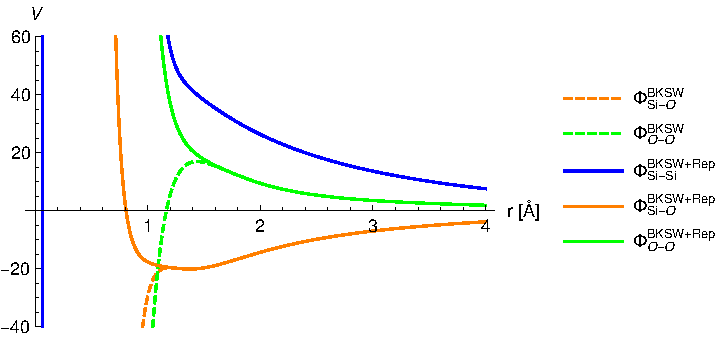
\includegraphics[]{chapters/chapter6/figures/BKSW.pdf}
    \caption{BKS potential with Wolf truncation.}
    \label{fig:BKS-potential}
\end{figure}

\subsection{Sample preparation}


\subsection{Quenching}

%%%%%%%%%%%%%%%%%%%%%%%%%%%%%%%%%%%%%%%%%%%%%
\section{Classical simulations: thermal conductivity}

\subsection{Cepstral analysis}
\paragraph{Dependence on cutoff frequency $f^*$}
(For the chosen sample at experimental density)
(comparison bw normal and vel-renormalized results)

\begin{figure}
    \centering
    \subfigure[\label{fig:csilica-sample-expdens-fstar-100ps}]{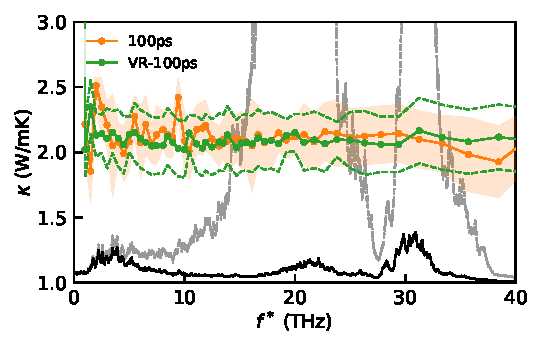
\includegraphics[width=8cm]{chapters/chapter6/figures/silica_expdens_kappa_fstar_VR_100ps.pdf}}
    \subfigure[\label{fig:csilica-sample-expdens-fstar-1ns}]{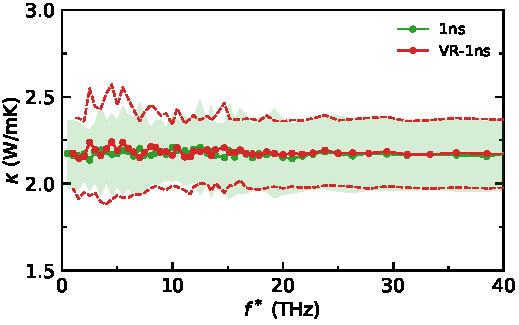
\includegraphics[width=8cm]{chapters/chapter6/figures/silica_expdens_kappa_fstar_VR_1ns.pdf}}
    \subfigure[\label{fig:csilica-sample-expdens-fstar-10ns}]{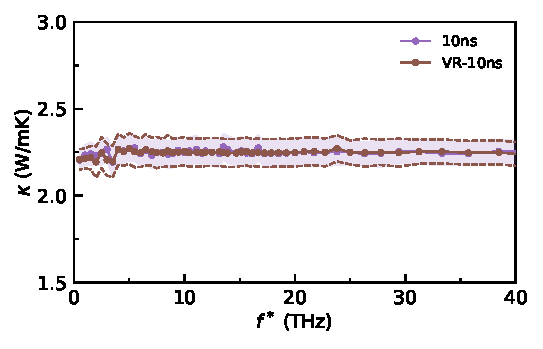
\includegraphics[width=8cm]{chapters/chapter6/figures/silica_expdens_kappa_fstar_VR_10ns.pdf}}
    \caption{Dependence of $\kappa$ on the choice of the cutoff frequency $f^*$, estimated from \emph{one} sample of (a) $100\un{ps}$, (b) $1\un{ns}$, and (c) $10\un{ps}$ of the ``original'' and VR heat flux time series. 
    The original and VR periodograms are reported for reference with grey and black lines, respectively.}
    \label{fig:csilica-sample-expdens-fstar}
\end{figure}
Fig.~\ref{fig:csilica-sample-expdens-fstar} -- stability of $\kappa$ as a function of $f^*$ increases with the length of the trajectory, as its predicted error decreases. The values and errors of $\kappa$ obtained from the VR time series are equivalent to the ones obtained from the original time series, and are slightly more stable with $f^*$. This is probably due to the much smaller power of the power spectrum of the VR heat flux, that may decrease the small artifacts introduced by the low-pass filter applied before resampling. 
Any frequency in the central region of the spectrum can be taken as $f^*$, hence we choose to set $f^*=28\un{THz}$. Conversely, a $f^*$ too small makes $\kappa$ deviate sensibly, due to the fact that the low-pass filter is not strong enough to avoid aliasing effects that modify the spectrum of the resampled time series; instead, a $f^*$ that is too high ($f^*\gtrsim 60\un{THz}$) induces a bias in $\kappa$, due to the fact the log-periodogram diverges to negative values and we start to have problems of numerical precision.

